%!TEX root = ../report.tex"
\section{Вопрос 58: Расширенная модель Take-Grant. Теорема об условиях реализации информационного потока на
запись. Алгоритм построения замыкания графа доступов расширенной модели Take-Grant и обоснование
его корректности.}

\textbf{Элементы расширенной модели Take-Grant:}
\begin{enumerate*}
		\item $ O $ -- множество объектов.
		\item $S \subseteq O$ -- множество субъектов.
		\item $ R = \{ r_1, \ldots, r_m \} \cup \{ t, g \} \cup \{r, w\} $ -- множество видов прав доступа, где t -- право брать права доступа, g -- давать, r -- читать, w -- писать.
		\item $ G = (S, O, E \cup F) $ -- конечный, ориентированный без петель граф доступов, $E \subseteq O \times O \times R $ -- реальные ребра графа, $ F \subseteq O \times O \times \{r, w\} $ -- мнимые ребра графа.
\end{enumerate*}

\textbf{Порядок перехода системы расширенной модели Take-Grant из состояния в состояние определяют де-юре и де-факто правила.}

\begin{figure}[H]
	\centering
	\begin{subfigure}[b]{0.4\textwidth}
		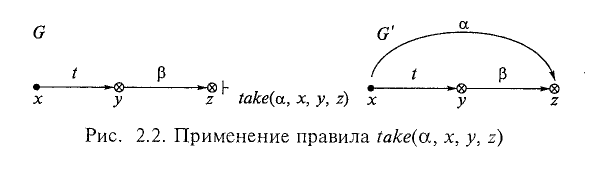
\includegraphics[width=\textwidth]{img/8.png}
		\captionsetup{labelformat=empty}
	\end{subfigure}
	%
	\begin{subfigure}[b]{0.4\textwidth}
		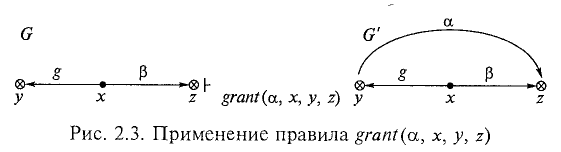
\includegraphics[width=\textwidth]{img/9.png}
		\captionsetup{labelformat=empty}
	\end{subfigure}
\end{figure}

\begin{figure}[H]
	\centering
	\begin{subfigure}[b]{0.4\textwidth}
		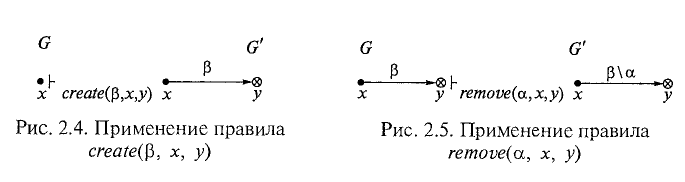
\includegraphics[width=\textwidth]{img/10.png}
		\captionsetup{labelformat=empty}
	\end{subfigure}
	%
	\begin{subfigure}[b]{0.4\textwidth}
		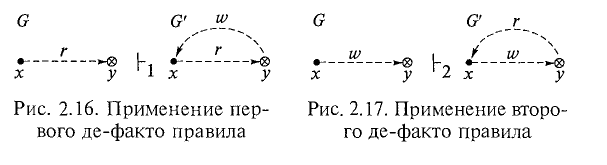
\includegraphics[width=\textwidth]{img/3.png}
		\captionsetup{labelformat=empty}
	\end{subfigure}
\end{figure}

\begin{figure}[H]
	\centering
	\begin{subfigure}[b]{0.4\textwidth}
		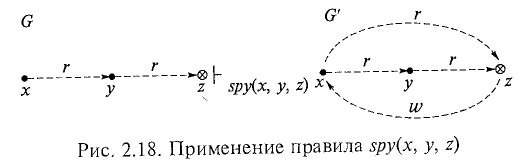
\includegraphics[width=\textwidth]{img/4.png}
		\captionsetup{labelformat=empty}
	\end{subfigure}
	%
	\begin{subfigure}[b]{0.4\textwidth}
		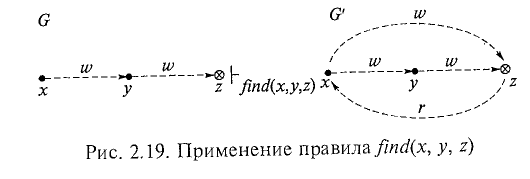
\includegraphics[width=\textwidth]{img/5.png}
		\captionsetup{labelformat=empty}
	\end{subfigure}
\end{figure}

\begin{figure}[H]
	\centering
	\begin{subfigure}[b]{0.4\textwidth}
		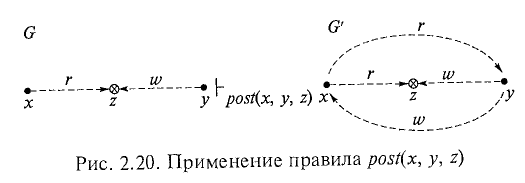
\includegraphics[width=\textwidth]{img/6.png}
		\captionsetup{labelformat=empty}
	\end{subfigure}
	%
	\begin{subfigure}[b]{0.4\textwidth}
		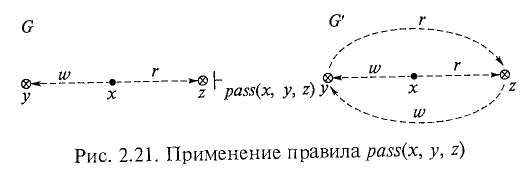
\includegraphics[width=\textwidth]{img/7.png}
		\captionsetup{labelformat=empty}
	\end{subfigure}
\end{figure}

\begin{defs}[Предикат can\_write]
	Пусть $x, y \in O_0, x \neq y,$ -- различные объекты графа доступов и информационных потоков $G_0 = (S_0, O_0, E_0 \cup F_0).$
	Определим предикат $can\_write(x, y, G_0)$, который будет истинным ТИТТК существуют графы
	$G_1 = (S_1, O_1, E_1 \cup F_1), \ldots, G_N = (S_N, O_N, E_N \cup F_N)$ и де-юре или де-факто правила
	$op_1, \ldots, op_N, N \geqslant 0 $ т.что $G_0 \vdash_{op_1} G_1 \vdash_{op_2} \ldots \vdash_{op_N} G_N$
	и $(x, y, w) \in F_N$.
\end{defs}

\begin{proofs}
	Пусть $G_0 = (S_0, O_0, E_0 \cup F_0)$ граф доступов и информационных потоков, $x,y \in O_0, x \neq y.$
	Тогда предикат $can\_write(x,y,G_0)$ истинен ТИТТК $\exists o_1, \ldots, o_m \in O_0$ где
	$o_1 = x, o_m = y$ т.что или $m = 2$ и $(x,y,w) \in F_0$, или для $i = 1, \ldots, m-1$ выполняется одно из условий:
	\begin{itemize*}
		\item $o_i \in S_0$ и или истинен предикат $can\_share(\{w\}, o_i, o_{i+1}, G_0)$, или $(o_i, o_{i+1}, w) \in E_0 \cup F_0$;
		\item $o_{i+1} \in S_0$ и или истинен предикат $can\_share(\{r\}, o_{i+1}, o_i, G_0)$, или $(o_{i+1}, o_i, r) \in E_0 \cup F_0$;
		\item $o_i,o_{i+1} \in S_0$ и или истинен предикат $can\_share(\alpha, o_i, o_{i+1}, G_0)$, или истенен предикат $can\_share(\alpha, o_{i+1}, o_i, G_0)$, где
		$\alpha \in \{t,g\}$, или $\exists o_i^{\shtrih} \in O_0$ т.что либо истинны предикаты $can\_share(\{t\}, o_i, o_i^{\shtrih}, G_0), can\_share(\{g\}, o_{i+1}, o_i^{\shtrih}, G_0)$
		либо истинны предикаты $can\_share(\{g\}, o_i, o_i^{\shtrih}, G_0), can\_share(\{t\}, o_{i+1}, o_i^{\shtrih}, G_0)$.
	\end{itemize*}
\end{proofs}

\begin{defs}[Замыкание графа]
	Пусть $G = (S, O, E \cup F)$ -- граф доступов $ $ и информационных потоков такой, что для каждого субъекта
	$s \in S \exists o \in O : (s,o,\{t,g,r,w\}) \subset E$. Тогда замыканием (или де-факто замыканием)
	графа $G$ называется граф доступов и информационных потоков $G^* = (S, O, E^* \cup F^*)$, полученный
	из $G$ применением последовательности правил take, grant и де-факто правил. При этом применениие к
	графу $G^*$ указанных правил не приводит к появлению новых ребер.
\end{defs}

\textbf{Алгоритм построения замыкания графа доступов состоит из трех этапов:}
\begin{enumerate*}
	\item Построение tg-замыкания
	\item Построение де-юре-замыкания
	\item Построение замыкания.
\end{enumerate*}

\begin{defs}[tg-замыкание графа]
	Пусть $G = (S, O, E \cup F)$ -- граф доступов и информационных потоков такой, что для каждого субъекта
	$s \in S \ \exists o \in O : (s,o,\{t,g,r,w\}) \subset E$. Тогда tg-замыканием
	графа $G$ называется граф доступов и информационных потоков $G^{tg} = (S, O, E^{tg} \cup F)$, полученный
	из $G$ применением последовательности правил take или grant. При этом каждое ребро $(o_1, o_2, \alpha)
	\in E^{tg} \diagdown E$ имеет вид $(o_1, o_2, t)$ или $(o_1, o_2, g)$, и применение к графу $G^{tg}$ правил
	take или grant не приводит к появлению новых ребер указанного вида.
\end{defs}

\begin{defs}[де-юре-замыкание графа]
	Пусть $G = (S, O, E \cup F)$ -- граф доступов и информационных потоков такой, что для каждого субъекта
	$s \in S \ \exists o \in O : (s,o,\{t,g,r,w\}) \subset E$. Тогда де-юре-замыканием
	графа $G$ называется граф доступов и информационных потоков $G^{де-юре} = (S, O, E^{\text{де-юре}} \cup F)$, полученный
	из $G$ применением последовательности правил take или grant. При этом применение к графу $G^{\text{де-юре}}$ правил
	take или grant не приводит к появлению в нем новых ребер.
\end{defs}

\textbf{Алгоритм построения tg-замыкания графа $G = (S,O,E \cup F)$:}
\begin{enumerate*}
	\item Для каждого $s \in S$ выполнить правило $create(\{t,g,r,w\}, s,o)$;
	при этом создаваемые объекты занести во множество $O$, создаваемые ребра во множество $E$.
	\item Инициализировать: $L = \{(x,y,\alpha) \in E, \alpha \in \{t,g\}\}$ -- список ребер
	графа и $N = \O$ -- множество вершин.
	\item Выбрать из $L$ первое ребро $(x,y,\alpha)$. Занести $x$ и $y$ во множество $N$.
	Удалить ребро $(x,y,\alpha)$ из списка $L$.
	\item Для всех вершин $z \in N$ проверить возможность применения правил $take$ или $grant$
	на тройке вершин $x,y,z$ с использованием ребра $(x,y,\alpha)$, выбранного на шаге 3.
	Если в результате применения правил take или grant появляются новые ребра вида $(a,b,\beta)$,
	где $\{a,b\} \subset \{x,y,z\}$ и $\beta \in \{t,g\}$, занести их в конец списка L и
	множество E.
	\item Пока список L не пуст, перейти на шаг 3.
\end{enumerate*}

\textbf{Алгоритм построения де-юре-замыкания графа $G = (S,O,E \cup F)$:}
\begin{enumerate*}
	\item Выполнить алгоритм tg-замыкания.
	\item Для каждой пары ребер вида $(x,y,t),(y,z,\alpha) \in E^{tg}, x \in S$, применить правило
	$take(\alpha, x, y, z)$ и, если полученное ребро $(x,z,\alpha) \notin E^{tg}$, то занести
	его во множество $E^{tg}$.
	\item Для каждой пары ребер вида $(x,y,g),(x,z,\alpha) \in E^{tg}, x \in S$, применить правило
	$grant(\alpha, x, y, z)$ и, если полученное ребро $(y,z,\alpha) \notin E^{tg}$, то занести
	его во множество $E^{tg}$.
	\item Для каждой пары ребер вида $(x,y,t),(y,z,\alpha) \in E^{tg}, x \in S$, применить правило
	$take(\alpha, x, y, z)$ и, если полученное ребро $(x,z,\alpha) \notin E^{tg}$, то занести
	его во множество $E^{tg}$.
\end{enumerate*}

\textbf{Алгоритм построения де-факто-замыкания графа $G = (S,O,E \cup F)$:}
\begin{enumerate*}
	\item Выполнить алгоритм де-юре-замыкания.
	\item Для всех ребер $(x,y,\alpha) \in E^{\text{де-юре}} \cup F, x \in S, \alpha \in \{w,r\}$,
	применить первые два де-факто правила. Если будут получены новые ребра, то занести их во
	множество F.
	\item Инициализировать: $L = \{(x,y,\alpha) \in E^{\text{де-юре}} \cup F,
	\alpha \in \{w,r\}\}$ -- список ребер графа и $N = \O$ -- множество вершин.
	\item Выбрать из $L$ первое ребро $(x,y,\alpha)$. Занести $x$ и $y$ во множество $N$.
	Удалить ребро $(x,y,\alpha)$ из списка $L$.
	\item Для всех вершин $z \in N$ проверить возможность применения де-факто правил
	на тройке вершин $x,y,z$ с использованием ребра $(x,y,\alpha)$.
	Если в результате применения де-факто правил spy, find, post, pass появляются новые
	ребра вида $(a,b,\beta)$, где $\{a,b\} \subset \{x,y,z\}$ и $\beta \in \{r,w\}$,
	занести их в конец списка L и множество F.
	\item Пока список L не пуст, перейти на шаг 4.
\end{enumerate*}

\begin{proofs}
	Все описанные выше алгоритмы построения замыкания корректны.
\end{proofs}
\newpage
